
\pdfminorversion=4 % for acroread
\documentclass[aspectratio=169,t,xcolor={usenames,dvipsnames}]{beamer}
%\documentclass[t,handout,xcolor={usenames,dvipsnames}]{beamer}
\usepackage{../beamerstyle}
\usepackage{dsfont}
\usepackage{bm}
\usepackage[english]{babel}
\usepackage[utf8]{inputenc}
\usepackage{graphicx}
\usepackage{algorithm}
\usepackage[ruled,vlined,algo2e,linesnumbered]{algorithm2e}
%\usepackage[boxed,vlined]{algorithm2e}
\usepackage{hyperref}
\usepackage{booktabs}
\usepackage{mathtools}

\usepackage{amsmath,amssymb}
\usepackage{listings}
\lstset{frame=lines,framesep=3pt,numbers=left,numberblanklines=false,basicstyle=\ttfamily\small}

\usepackage{subfig}
\usepackage{multicol}
%\usepackage{appendixnumberbeamer}
%
\usepackage{tcolorbox}

\usepackage{pgfplots}
\usepackage{tikz}
\usetikzlibrary{trees} 
\usetikzlibrary{shapes.geometric}
\usetikzlibrary{positioning,shapes,shadows,arrows,calc,mindmap}
\usetikzlibrary{positioning,fadings,through}
\usetikzlibrary{decorations.pathreplacing}
\usetikzlibrary{intersections}
\usetikzlibrary{positioning,fit,calc,shadows,backgrounds}
\pgfdeclarelayer{background}
\pgfdeclarelayer{foreground}
\pgfsetlayers{background,main,foreground}
\tikzstyle{activity}=[rectangle, draw=black, rounded corners, text centered, text width=8em]
\tikzstyle{data}=[rectangle, draw=black, text centered, text width=8em]
\tikzstyle{myarrow}=[->, thick, draw=black]

% Define the layers to draw the diagram
\pgfdeclarelayer{background}
\pgfdeclarelayer{foreground}
\pgfsetlayers{background,main,foreground}

%\usepackage{listings}
%\lstset{numbers=left,
%  showstringspaces=false,
%  frame={tb},
%  captionpos=b,
%  lineskip=0pt,
%  basicstyle=\ttfamily,
%%  extendedchars=true,
%  stepnumber=1,
%  numberstyle=\small,
%  xleftmargin=1em,
%  breaklines
%}

 
\definecolor{blue}{RGB}{0, 74, 153}

\usetheme{Boadilla}
%\useinnertheme{rectangles}
\usecolortheme{whale}
\setbeamercolor{alerted text}{fg=blue}
\useoutertheme{infolines}
\setbeamertemplate{navigation symbols}{\vspace{-5pt}} % to lower the logo
\setbeamercolor{date in head/foot}{bg=white} % blue
\setbeamercolor{date in head/foot}{fg=white}
\setbeamercolor{author  in head/foot}{bg=white} %blue
\setbeamercolor{title in head/foot}{bg=white} % blue
\setbeamercolor{title}{fg=white, bg=blue}
\setbeamercolor{block title}{fg=white,bg=blue}
\setbeamercolor{block body}{bg=blue!10}
\setbeamercolor{frametitle}{fg=white, bg=blue}
\setbeamercovered{invisible}

\makeatletter
\setbeamertemplate{footline}
{
  \leavevmode%
  \hbox{%
  \begin{beamercolorbox}[wd=.333333\paperwidth,ht=2.25ex,dp=1ex,center]{author in head/foot}%
%    \usebeamerfont{author in head/foot}\insertshortauthor
  \end{beamercolorbox}%
  \begin{beamercolorbox}[wd=.333333\paperwidth,ht=2.25ex,dp=1ex,center]{title in head/foot}%
    \usebeamerfont{title in head/foot}\insertshorttitle
  \end{beamercolorbox}%
  \begin{beamercolorbox}[wd=.333333\paperwidth,ht=2.25ex,dp=1ex,right]{date in head/foot}%
    \usebeamerfont{date in head/foot}\insertshortdate{}\hspace*{2em}
%    \insertframenumber\hspace*{2ex} 
  \end{beamercolorbox}}%
  \vskip0pt%
}
\makeatother

%\pgfdeclareimage[height=1.2cm]{automl}{images/logos/automl.png}
%\pgfdeclareimage[height=1.2cm]{freiburg}{images/logos/freiburg}

%\logo{\pgfuseimage{freiburg}}

\newcommand{\comment}[1]{
	\noindent
	%\vspace{0.25cm}
	{\color{red}{\textbf{TODO:} #1}}
	%\vspace{0.25cm}
}
\renewcommand{\comment}[1]{}
\newcommand{\hide}[1]{}
\newcommand{\cemph}[2]{\emph{\textcolor{#1}{#2}}}

\newcommand{\lit}[1]{{\footnotesize\color{black!70}[#1]}}

\newcommand{\litw}[1]{{\footnotesize\color{black!20}[#1]}}


\newcommand{\myframe}[2]{\begin{frame}[c]{#1}#2\end{frame}}
\newcommand{\myframetop}[2]{\begin{frame}{#1}#2\end{frame}}
\newcommand{\myit}[1]{\begin{itemize}#1\end{itemize}}
\newcommand{\myblock}[2]{\begin{block}{#1}#2\end{block}}


\newcommand{\votepurple}[1]{\textcolor{Purple}{$\bigstar$}}
\newcommand{\voteyellow}[1]{\textcolor{Goldenrod}{$\bigstar$}}
\newcommand{\voteblue}[1]{\textcolor{RoyalBlue}{$\bigstar$}}
\newcommand{\votepink}[1]{\textcolor{Pink}{$\bigstar$}}

\newcommand{\diff}{\mathop{}\!\mathrm{d}}
\newcommand{\refstyle}[1]{{\small{\textcolor{gray}{#1}}}}
\newcommand{\hands}[0]{\includegraphics[height=1.5em]{images/hands}}
\newcommand{\transpose}[0]{{\textrm{\tiny{\sf{T}}}}}
\newcommand{\norm}{{\mathcal{N}}}
\newcommand{\cutoff}[0]{\kappa}
\newcommand{\instD}[0]{\dataset}
\newcommand{\insts}[0]{\mathcal{I}}
\newcommand{\inst}[0]{i}
\newcommand{\pcs}[0]{\mathbf{\Lambda}}
\newcommand{\bx}[0]{\conf}
\newcommand{\conf}[0]{\mathbf{\lambda}}
\newcommand{\defconf}[0]{\mathbf{\lambda}_{\text{def}}}
\newcommand{\finconf}[0]{\mathbf{\lambda}^*}
\newcommand{\incumbent}[0]{\finconf}
\newcommand{\confs}[0]{\pcs}
%\newcommand{\vlambda}[0]{\bm{\lambda}}
%\newcommand{\vLambda}[0]{\bm{\Lambda}}
\newcommand{\dataset}[0]{\mathcal{D}}
\newcommand{\datasets}[0]{\mathbf{D}}
\newcommand{\loss}[0]{\mathcal{L}}

% \renewcommand{\vec}[1]{\mathbf{#1}}
\newcommand{\hist}[0]{\mathcal{H}}
\newcommand{\param}[0]{p}
\newcommand{\algo}[0]{\mathcal{A}}
\newcommand{\algos}[0]{\mathbf{A}}
%\newcommand{\nn}[0]{N}
\newcommand{\feats}[0]{\mathcal{F}}
\newcommand{\feat}[0]{\vec{f}}
\newcommand{\cluster}[0]{\vec{h}}
\newcommand{\clusters}[0]{\vec{H}}
\newcommand{\perf}[0]{\mathbb{R}}
%\newcommand{\surro}[0]{\mathcal{S}}
\newcommand{\surro}[0]{\hat{f}}
\newcommand{\func}[0]{f}
\newcommand{\epm}[0]{\surro}
\newcommand{\portfolio}[0]{\mathcal{P}}
\newcommand{\schedule}[0]{\mathcal{S}}
\newcommand{\mdata}[0]{\dataset_{\text{meta}}}

% Deep Learning
\newcommand{\weights}[0]{\theta}
\newcommand{\metaweights}[0]{\phi}


% reinforcement learning
\newcommand{\policies}[0]{\Pi}
\newcommand{\policy}[0]{\pi}
\newcommand{\actionRL}[0]{a}
\newcommand{\stateRL}[0]{s}
\newcommand{\statesRL}[0]{\mathcal{S}}
\newcommand{\rewardRL}[0]{r}
\newcommand{\rewardfuncRL}[0]{\mathcal{R}}

\RestyleAlgo{algoruled}
\DontPrintSemicolon
\LinesNumbered
\SetAlgoVlined
\SetFuncSty{textsc}

\SetKwInOut{Input}{Input}
\SetKwInOut{Output}{Output}
\SetKw{Return}{return}

%\newcommand{\changed}[1]{{\color{red}#1}}

%\newcommand{\citeN}[1]{\citeauthor{#1}~(\citeyear{#1})}

\renewcommand{\vec}[1]{\mathbf{#1}}
\DeclareMathOperator*{\argmin}{arg\,min}
\DeclareMathOperator*{\argmax}{arg\,max}

\newcommand{\aqme}{\textit{AQME}}
\newcommand{\aslib}{\textit{ASlib}}
\newcommand{\llama}{\textit{LLAMA}}
\newcommand{\satzilla}{\textit{SATzilla}}
\newcommand{\satzillaY}[1]{\textit{SATzilla'{#1}}}
\newcommand{\snnap}{\textit{SNNAP}}
\newcommand{\claspfolioTwo}{\textit{claspfolio~2}}
\newcommand{\flexfolio}{\textit{FlexFolio}}
\newcommand{\claspfolioOne}{\textit{claspfolio~1}}
\newcommand{\isac}{\textit{ISAC}}
\newcommand{\eisac}{\textit{EISAC}}
\newcommand{\sss}{\textit{3S}}
\newcommand{\sunny}{\textit{Sunny}}
\newcommand{\ssspar}{\textit{3Spar}}
\newcommand{\cshc}{\textit{CSHC}}  
\newcommand{\cshcpar}{\textit{CSHCpar}}  
\newcommand{\measp}{\textit{ME-ASP}} 
\newcommand{\aspeed}{\textit{aspeed}}
\newcommand{\autofolio}{\textit{AutoFolio}}
\newcommand{\cedalion}{\textit{Cedalion}}
\newcommand{\fanova}{\textit{fANOVA}}
\newcommand{\sbs}{\textit{SB}}
\newcommand{\oracle}{\textit{VBS}}

% like approaches
\newcommand{\claspfoliolike}[1]{\texttt{claspfolio-#1-like}}
\newcommand{\satzillalike}[1]{\texttt{SATzilla'#1-like}}
\newcommand{\isaclike}{\texttt{ISAC-like}}
\newcommand{\ssslike}{\texttt{3S-like}}
\newcommand{\measplike}{\texttt{ME-ASP-like}}

\newcommand{\aspCoseal}{\textit{ASP-POTASSCO}}
\newcommand{\cspCoseal}{\textit{CSP-2010}}
\newcommand{\maxsatCoseal}{\textit{MAXSAT12-PMS}}
\newcommand{\premarCoseal}{\textit{PRE\-MARSHALLING}}
\newcommand{\qbfCoseal}{\textit{QBF-2011}}
\newcommand{\satallTwelveCoseal}{\textit{SAT12-ALL}}
\newcommand{\sathandTwelveCoseal}{\textit{SAT12-HAND}}
\newcommand{\satinduTwelveCoseal}{\textit{SAT12-INDU}}
\newcommand{\satrandTwelveCoseal}{\textit{SAT12-RAND}}
\newcommand{\sathandElevenCoseal}{\textit{SAT11-HAND}}
\newcommand{\satinduElevenCoseal}{\textit{SAT11-INDU}}
\newcommand{\satrandElevenCoseal}{\textit{SAT11-RAND}}
\newcommand{\proteusCoseal}{\textit{PROTEUS-2014}}

\newcommand{\irace}{\textit{I/F-race}}
\newcommand{\gga}{\textit{GGA}}
\newcommand{\smac}{\textit{SMAC}}
\newcommand{\paramils}{\textit{ParamILS}}
\newcommand{\spearmint}{\textit{Spearmint}}
\newcommand{\tpe}{\textit{TPE}}

\newcommand{\gringo}{\textit{gringo}}
\newcommand{\clasp}{\textit{clasp}}
\newcommand{\lingeling}{\textit{lingeling}}

\newcommand{\hydra}{\textit{Hydra}}

\newcommand{\plingeling}{\textit{Plingeling}}
\newcommand{\ccasat}{\textit{CCASat}}

\usepackage{pifont}
\newcommand{\itarrow}{\mbox{\Pisymbol{pzd}{229}}}
\newcommand{\ithook}{\mbox{\Pisymbol{pzd}{52}}}
\newcommand{\itcross}{\mbox{\Pisymbol{pzd}{56}}}
\newcommand{\ithand}{\mbox{\raisebox{-1pt}{\Pisymbol{pzd}{43}}}}

%\DeclareMathOperator*{\argmax}{arg\,max}

\newcommand{\ie}{{\it{}i.e.\/}}
\newcommand{\eg}{{\it{}e.g.\/}}
\newcommand{\cf}{{\it{}cf.\/}}
\newcommand{\wrt}{\mbox{w.r.t.}}
\newcommand{\vs}{{\it{}vs\/}}
\newcommand{\vsp}{{\it{}vs\/}}
\newcommand{\etc}{{\copyedit{etc.}}}
\newcommand{\etal}{{\it{}et al.\/}}

\newcommand{\pscProc}{{\bf procedure}}
\newcommand{\pscBegin}{{\bf begin}}
\newcommand{\pscEnd}{{\bf end}}
\newcommand{\pscEndIf}{{\bf endif}}
\newcommand{\pscFor}{{\bf for}}
\newcommand{\pscEach}{{\bf each}}
\newcommand{\pscThen}{{\bf then}}
\newcommand{\pscElse}{{\bf else}}
\newcommand{\pscWhile}{{\bf while}}
\newcommand{\pscIf}{{\bf if}}
\newcommand{\pscRepeat}{{\bf repeat}}
\newcommand{\pscUntil}{{\bf until}}
\newcommand{\pscWithProb}{{\bf with probability}}
\newcommand{\pscOtherwise}{{\bf otherwise}}
\newcommand{\pscDo}{{\bf do}}
\newcommand{\pscTo}{{\bf to}}
\newcommand{\pscOr}{{\bf or}}
\newcommand{\pscAnd}{{\bf and}}
\newcommand{\pscNot}{{\bf not}}
\newcommand{\pscFalse}{{\bf false}}
\newcommand{\pscEachElOf}{{\bf each element of}}
\newcommand{\pscReturn}{{\bf return}}

%\newcommand{\param}[1]{{\sl{}#1}}
\newcommand{\var}[1]{{\it{}#1}}
\newcommand{\cond}[1]{{\sf{}#1}}
%\newcommand{\state}[1]{{\sf{}#1}}
%\newcommand{\func}[1]{{\sl{}#1}}
\newcommand{\set}[1]{{\Bbb #1}}
%\newcommand{\inst}[1]{{\tt{}#1}}
\newcommand{\myurl}[1]{{\small\sf #1}}

\newcommand{\Nats}{{\Bbb N}}
\newcommand{\Reals}{{\Bbb R}}
\newcommand{\extset}[2]{\{#1 \; | \; #2\}}

\newcommand{\vbar}{$\,\;|$\hspace*{-1em}\raisebox{-0.3mm}{$\,\;\;|$}}
\newcommand{\vendbar}{\raisebox{+0.4mm}{$\,\;|$}}
\newcommand{\vend}{$\,\:\lfloor$}


\newcommand{\goleft}[2][.7]{\parbox[t]{#1\linewidth}{\strut\raggedright #2\strut}}
\newcommand{\rightimage}[2][.3]{\mbox{}\hfill\raisebox{1em-\height}[0pt][0pt]{\includegraphics[width=#1\linewidth]{#2}}\vspace*{-\baselineskip}}







\title[AutoML: Overview]{AutoML: Automated Machine Learning}
\subtitle{Algorithm Selection}
\author[Lars Kotthoff]{Bernd Bischl \and Frank Hutter \and \underline{Lars Kotthoff} \and Marius Lindauer}
\institute{}
\date{}



% \AtBeginSection[] % Do nothing for \section*
% {
%   \begin{frame}{Outline}
%     \bigskip
%     \vfill
%     \tableofcontents[currentsection]
%   \end{frame}
% }

\def\blfootnote{}

\begin{document}
	
	\maketitle
	

%----------------------------------------------------------------------
%----------------------------------------------------------------------

%----------------------------------------------------------------------
\begin{frame}[c]{Algorithm Selection}
    \begin{center}
        \Large{Given a problem, choose the best algorithm to solve it.}
    \end{center}
    \blfootnote{Rice, John R. ``The Algorithm Selection Problem.'' Advances in
    Computers 15 (1976): 65–118.}
\end{frame}

\begin{frame}[c]{Algorithm Selection}
\begin{block}{More formally}
        Let 
        \begin{itemize}
                \item $p(\dataset)$ be a probability distribution over datasets $\dataset \in \datasets$,
                \item $\portfolio$ a portfolio of algorithms $\algo \in \portfolio$, and
                \item $\cost: \portfolio \times \datasets \rightarrow \perf$ be a cost metric   
        \end{itemize}
        
        the \emph{per-instance algorithm selection problem} is to obtain a mapping 
        $s: \dataset \mapsto \algo$ 
        such that
        $$\argmin_{s} \int_{\datasets} \cost(s(\dataset),\dataset) p(\dataset) \diff\dataset$$
\end{block}

\end{frame}
%-----------------------------------------------------------------------

\begin{frame}{Motivation: Performance Differences}
\begin{center}
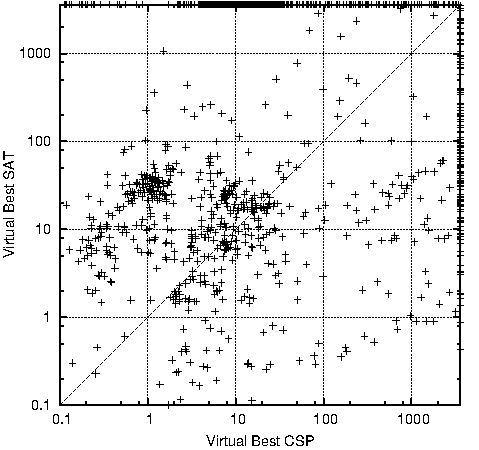
\includegraphics[height=.7\textheight]{csp_v_sat}
\end{center}
\blfootnote{Hurley, Barry, Lars Kotthoff, Yuri Malitsky, and Barry O’Sullivan.
``Proteus: A Hierarchical Portfolio of Solvers and Transformations.'' In CPAIOR,
2014.}
\end{frame}

\begin{frame}{Motivation: Leveraging the Differences}
\begin{center}
\includegraphics[height=.7\textheight]{satzilla}
\end{center}
\blfootnote{Xu, Lin, Frank Hutter, Holger H. Hoos, and Kevin Leyton-Brown.
``SATzilla: Portfolio-Based Algorithm Selection for SAT.'' J. Artif. Intell.
Res. (JAIR) 32 (2008): 565–606.}
\end{frame}

\begin{frame}{Algorithm Selection}
\begin{center}
\resizebox{.7\textwidth}{!}{%
\tikzset{>=latex}
\begin{tikzpicture}[node distance=1em,inner sep=.5em,n/.style={drop
shadow,fill=white,rounded corners},scale=.5]
\node (p) [align=left] {Portfolio};
\node (a2) [rectangle,align=center,below=of p,draw] {Algorithm 2};
\node (a1) [rectangle,align=center,left=of a2,draw] {Algorithm 1};
\node (a3) [rectangle,align=center,right=of a2,draw] {Algorithm 3};
\begin{pgfonlayer}{background}
\node (pc) [n,fit={(p) (a1) (a2) (a3)},draw] {};
\end{pgfonlayer}

\node (i) [align=left,right=15em of p.east] {Training Instances};
\node (i2) [rectangle,align=center,below=of i,draw] {Instance 2};
\node (i1) [rectangle,align=center,left=of i2,draw] {Instance 1};
\node (i3) [rectangle,align=center,right=of i2,draw] {Instance 3};
\begin{pgfonlayer}{background}
\node (ic) [n,fit={(i) (i1) (i2) (i3)},draw] {};
\end{pgfonlayer}

\node (as) [n,draw,align=left,below=10em of $(p)!0.5!(i)$] {Algorithm Selection};
\node (m) [n,draw,align=left,below=3em of as] {Performance Model};

\node (it) [align=center,right=10em of m] {Instance 4\\Instance 5\\Instance 6\\$\vdots$};

\node (s) [align=center,below=3em of m] {Instance 4: Algorithm 2\\Instance 5: Algorithm 3\\Instance 6: Algorithm 3\\$\vdots$};

\path [->] (pc.south) edge (as);
\path [->] (ic.south) edge node [below right] {Feature Extraction} (as);
\path [->] ([xshift=-.5em]it.west) edge node [below,align=center] {Feature\\Extraction} (m.east);
\path [->] (as.south) edge (m.north);
\path [->] (m.south) edge (s.north);
\end{tikzpicture}}
\end{center}
\end{frame}

\begin{frame}{Algorithm Portfolios}
\begin{itemize}
\item instead of a single algorithm, use several complementary algorithms
\item idea from Economics -- minimise risk by spreading it out across several
    securities
\item same for computational problems -- minimise risk of algorithm performing
    poorly
\item in practice often constructed from competition winners
\end{itemize}
\blfootnote{Huberman, Bernardo A., Rajan M. Lukose, and Tad Hogg. “An Economics
Approach to Hard Computational Problems.” Science 275, no. 5296 (1997): 51–54.
doi:10.1126/science.275.5296.51.}
\end{frame}

\begin{frame}{Algorithms}
``algorithm'' used in a very loose sense
\begin{itemize}
\item constraint solvers
\item search strategies
\item modelling choices
\item different types of consistency
\end{itemize}
\end{frame}

\begin{frame}{Evaluation of Portfolios}
\begin{itemize}
\item single best algorithm
    \begin{itemize}
    \item algorithm with the best performance across all instances
    \item lower bound for performance of portfolio -- hopefully we are better!
    \end{itemize}
\item virtual best algorithm
    \begin{itemize}
    \item choose the best algorithm for each instance
    \item corresponds to oracle predictor or overhead-free parallel portfolio
    \item upper bound on portfolio performance (assuming robust performance
    measurements) -- note difference to configuration
    \end{itemize}
\end{itemize}
\end{frame}

\begin{frame}{Parallel Portfolios}
Why not simply run all algorithms in parallel?
\begin{itemize}
\item not enough resources may be available/waste of resources
\item algorithms may be parallelized themselves
\item memory contention
\item \ldots
\end{itemize}
\end{frame}

\begin{frame}{Building an Algorithm Selection System}
\begin{itemize}
\item most approaches rely on machine learning
\item train with representative data, i.e.\ performance of all algorithms in
    portfolio on a number of instances
\item evaluate performance on separate set of instances
\item potentially large amount of prep work
\end{itemize}
\end{frame}

\begin{frame}{Choosing Instances}
\begin{itemize}
\item we want selectors that generalise, i.e.\ good for more than one
instance
\item split instances into training set (which we configure on) and test set
(which we only evaluate performance on)
\item need to balance easy/hard instances in both sets
\item may need hundreds or thousands of instances
\end{itemize}
\end{frame}

\begin{frame}{Key Components of an Algorithm Selection System}
\begin{itemize}
\item feature extraction
\item performance model
\item prediction-based selector/scheduler
\end{itemize}
optional:
\begin{itemize}
\item presolver
\item secondary/hierarchical models and predictors (e.g.\ for feature extraction
    time)
\end{itemize}
\end{frame}

\begin{frame}{Features}
\begin{itemize}
\item relate properties of problem instances to performance
\item relatively cheap to compute
\item specified by domain expert
\item syntactic -- analyse instance description
\item probing -- run algorithm for short time
\item dynamic -- instance changes while algorithm is running
\end{itemize}
\end{frame}

\begin{frame}{Syntactic Features}
\begin{itemize}
\item number of variables, number of clauses/constraints/\ldots
\item ratios
\item order of variables/values
\item clause/constraints--variable graph or variable graph:
    \begin{itemize}
    \item node degrees
    \item connectivity
    \item clustering coefficient
    \item \ldots
    \end{itemize}
\item \ldots
\end{itemize}
\end{frame}

\begin{frame}{Probing Features}
\begin{itemize}
\item number of nodes/propagations within time limit
\item estimate of search space size
\item tightness of problem/constraints
\item \ldots
\end{itemize}
\end{frame}

\begin{frame}{Dynamic Features}
\begin{itemize}
\item change of variable domains
\item number of constraint propagations
\item number of failures a clause participated in
\item \ldots
\end{itemize}
\end{frame}

\begin{frame}{What Features do we need in Practice?}
\begin{itemize}
\item trade-off between complex features and complex models
\item in practice, very simple features (e.g.\ problem size) can perform well
\item in the end, whatever works best
\end{itemize}
\end{frame}

\begin{frame}{Types of Performance Models}
\begin{itemize}
\item models for entire portfolios
\item models for individual algorithms
\item models that are somewhere in between (e.g.\ pairs of algorithms)
\end{itemize}
\end{frame}

\begin{frame}{Models for Entire Portfolios}
\begin{itemize}
\item predict the best algorithm in the portfolio
\item alternatively: cluster and assign best algorithms to clusters
\end{itemize}
optional (but important):
\begin{itemize}
\item attach a ``weight'' during learning (e.g.\ the difference between best
    and worst solver) to bias model towards the ``important'' instances
\item special loss metric
\end{itemize}
\blfootnote{Gent, Ian P., Christopher A. Jefferson, Lars Kotthoff, Ian Miguel,
Neil Moore, Peter Nightingale, and Karen E. Petrie. ``Learning When to Use Lazy
Learning in Constraint Solving.'' In 19th European Conference on Artificial
Intelligence, 873–78, 2010.}
\blfootnote{Kadioglu, Serdar, Yuri Malitsky, Meinolf Sellmann, and Kevin
Tierney. ``ISAC – Instance-Specific Algorithm Configuration.'' In 19th European
Conference on Artificial Intelligence, 751–56, 2010.}
\end{frame}

\begin{frame}{Models for Individual Algorithms}
\begin{itemize}
\item predict the performance for each algorithm separately
\item combine the predictions to choose the best one
\item for example: predict the runtime for each algorithm, choose the one with
    the lowest runtime
\end{itemize}
\blfootnote{Xu, Lin, Frank Hutter, Holger H. Hoos, and Kevin Leyton-Brown.
``SATzilla: Portfolio-Based Algorithm Selection for SAT.'' J. Artif. Intell.
Res. (JAIR) 32 (2008): 565–606.}
\end{frame}

\begin{frame}{Hybrid Models}
\begin{itemize}
\item get the best of both worlds
\item for example: consider pairs of algorithms to take relations into account
\item for each pair of algorithms, learn model that predicts which one is faster
\end{itemize}
\blfootnote{Xu, Lin, Frank Hutter, Holger H. Hoos, and Kevin Leyton-Brown.
``Hydra-MIP: Automated Algorithm Configuration and Selection for Mixed Integer
Programming.'' In RCRA Workshop on Experimental Evaluation of Algorithms for
Solving Problems with Combinatorial Explosion at the International Joint
Conference on Artificial Intelligence (IJCAI), 16–30, 2011.}
\blfootnote{Kotthoff, Lars. ``Hybrid Regression-Classification Models for
Algorithm Selection.'' In 20th European Conference on Artificial Intelligence,
480–85, 2012.}
\end{frame}

\begin{frame}{Types of Performance Models}
\begin{center}
\resizebox{!}{.8\textheight}{%
\tikzset{>=latex}
\begin{tikzpicture}[node distance=1em,inner sep=.5em,n/.style={drop shadow,fill=white,rounded corners}
]

\node (pm2c) [n,align=center,draw] {Regression Models\\
\begin{tikzpicture}[scale=0.3]
\draw (0,1) .. controls (1,1) .. (4,0) node [right]{A1};
\draw (0,0) .. controls (1,0) .. (4,4) node [right]{A2};
\draw (0,2) .. controls (2,3) .. (4,2) node [right]{A3};
\end{tikzpicture}
};

\node (pm2cr) [align=left,right=3em of pm2c] {A1: 1.2\\\textbf{A2: 4.5}\\A3: 3.9};

\node (pm1c) [n,align=center,above=of pm2c,draw] {Classification Model\\[1em]
\begin{tikzpicture}[scale=0.3,sibling distance=8em,every node/.style={circle,fill=black,inner sep=.2em}]
\node (pm1) [draw] {}
child{ node [draw] {}
        child{ node [draw,label={below left:A1}] {} }
        child{ node [draw] {}
                        child{ node [draw,label={below:A3}] {}}
                        child{ node [draw,label={below:A1}] {}}
        }
}
child{ node [draw,label={below right:A2}] {} }
;
\end{tikzpicture}
};

\node (pm1cr) [align=left,right=3em of pm1c] {\textbf{A1}};

\node (pm3c) [n,align=center,below=of pm2c,draw] {Pairwise Classification Models\\[1em]
\begin{tikzpicture}[scale=0.3,every label/.append style={shape=rectangle},sibling distance=3em,every node/.style={circle,fill=black,inner sep=.2em}]
\node [draw,label={above:A1 vs.\ A2}] {}
child{ node [draw] {}
        child{ node [draw,label={below left:A1}] {} }
        child{ node [draw] {}
                        child{ node [draw,label={below left:A2}] {}}
                        child{ node [draw,label={below right:A1}] {}}
        }
}
child{ node [draw,label={below right:A1}] {} }
;
\end{tikzpicture}
\hspace{1em}
\begin{tikzpicture}[scale=0.3,every label/.append style={shape=rectangle},sibling distance=3em,every node/.style={circle,fill=black,inner sep=.2em}]
\node [draw,label={above:A1 vs.\ A3}] {}
child{ node [draw] {}
        child{ node [draw,label={below left:A1}] {} }
        child{ node [draw] {}
                        child{ node [draw,label={below left:A1}] {}}
                        child{ node [draw,label={below right:A3}] {}}
        }
}
child{ node [draw,label={below right:A3}] {} }
;
\end{tikzpicture}
\hspace{1em}
\raisebox{3.7em}{\ldots}
};

\node (pm3cr) [align=left,right=1em of pm3c] {A1: 1 vote\\A2: 0 votes\\\textbf{A3: 2 votes}};

\node (pm4c) [n,align=center,below=of pm3c,draw] {Pairwise Regression Models\\[1em]
\begin{tikzpicture}[scale=0.3]
\draw (2,6) node {A1 - A2};
\draw (0,3) .. controls (1,1) .. (4,0);
\draw (0,2) -- (4,2) node [right] {0};
\end{tikzpicture}
\hspace{1em}
\begin{tikzpicture}[scale=0.3]
\draw (2,6) node {A1 - A3};
\draw (0,0) .. controls (1,0) .. (4,4);
\draw (0,2) -- (4,2) node [right] {0};
\end{tikzpicture}
\hspace{1em}
\raisebox{2em}{\ldots}
};

\node (pm4cr) [align=left,right=1em of pm4c] {A1: -1.3\\A2: 0.4\\\textbf{A3: 1.7}};

\node (pmc) [fit={(pm1c) (pm1cr) (pm2c) (pm2cr) (pm3c) (pm3cr) (pm4c) (pm4cr)},draw,dashed] {};

\node (it) [align=center,left=3em of pmc] {Instance 1\\Instance 2\\Instance 3\\$\vdots$};

\node (ps) [align=center,right=3em of pmc] {Instance 1: Algorithm 2\\Instance 2:
Algorithm 1\\Instance 3: Algorithm 3\\$\vdots$};

\path [->] (it) edge (pmc);
\path [->] (pmc) edge (ps);
\path [->] (pm1c) edge (pm1cr);
\path [->] (pm2c) edge (pm2cr);
\path [->] (pm3c) edge (pm3cr);
\end{tikzpicture}}
\end{center}
\end{frame}

\begin{frame}{Types of Predictions/Algorithm Selectors}
\begin{itemize}
\item best algorithm
\item $n$ best algorithms ranked
\item allocation of resources to $n$ algorithms
\item change the currently running algorithm?
\end{itemize}
\blfootnote{Kotthoff, Lars. ``Ranking Algorithms by Performance.'' In LION 8,
2014.}
\blfootnote{Kadioglu, Serdar, Yuri Malitsky, Ashish Sabharwal, Horst Samulowitz,
and Meinolf Sellmann. ``Algorithm Selection and Scheduling.'' In 17th
International Conference on Principles and Practice of Constraint Programming,
454–69, 2011.}
\blfootnote{Stergiou, Kostas. ``Heuristics for Dynamically Adapting Propagation
in Constraint Satisfaction Problems.'' AI Commun. 22, no. 3 (2009): 125–41.}
\end{frame}

\begin{frame}{Time of Prediction}
\begin{itemize}
\item before problem is being solved
    \begin{itemize}
    \item select algorithm(s) once
    \item no recourse if predictions are bad
    \end{itemize}
\item while problem is being solved
    \begin{itemize}
    \item continuously monitor problem features and/or performance
    \item can remedy bad initial choice or react to changing problem
    \end{itemize}
\end{itemize}
\end{frame}

\begin{frame}{Example System -- SATzilla}
\begin{itemize}
\item portfolio of 7 SAT solvers, trained on 4811 problem instances
\item syntactic (33) and probing features (15)
\item ridge regression to predict log runtime for each solver, choose the solver with the best predicted performance
\item later version uses random forests to predict better algorithm for each
 pair, aggregation through simple voting scheme
\item pre-solving, feature computation time prediction, hierarchical model,
selection of algorithms to include in portfolio based on overall performance
\item won several competitions
\end{itemize}
\blfootnote{Xu, Lin, Frank Hutter, Holger H. Hoos, and Kevin Leyton-Brown.
``SATzilla: Portfolio-Based Algorithm Selection for SAT.'' J. Artif. Intell.
Res. (JAIR) 32 (2008): 565–606.}
\end{frame}

\begin{frame}{Benchmark library -- ASlib}
\begin{itemize}
\item \url{https://github.com/coseal/aslib_data}
\item currently 17 data sets/scenarios with more in preparation
\item SAT, CSP, QBF, ASP, MAXSAT, OR
\item includes data used frequently in the literature that you may want to
    evaluate your approach on
\item more scenarios in the pipeline
\item \url{http://aslib.net}\\[1em]
\end{itemize}
\blfootnote{
Bischl, Bernd, Pascal Kerschke, Lars Kotthoff, Marius Lindauer, Yuri Malitsky,
Alexandre Fréchette, Holger H. Hoos, et al. ``ASlib: A Benchmark Library for
Algorithm Selection.'' Artificial Intelligence Journal (AIJ), no. 237 (2016): 41–58.
}
\end{frame}

\begin{frame}{Tools}
\begin{description}
\item[autofolio] \url{https://bitbucket.org/mlindauer/autofolio/}
\item[LLAMA] \url{https://bitbucket.org/lkotthoff/llama}
\item[SATzilla]
 \footnotesize{\url{http://www.cs.ubc.ca/labs/beta/Projects/SATzilla/}}
\end{description}
\end{frame}

\begin{frame}{(Much) More Information}
\begin{center}
\includegraphics[height=.6\textheight]{survey}\\
\url{http://larskotthoff.github.io/assurvey/}
\end{center}
\blfootnote{Kotthoff, Lars. ``Algorithm Selection for Combinatorial Search
Problems: A Survey.'' AI Magazine 35, no. 3 (2014): 48–60.}
\end{frame}

\end{document}
